\section{Design of the system [VI]}

Architecture of our system essentially repeats common design of the Speed layer, described in the Section~\ref{sec:speed_layer}.
The system consists of three main components: data source, data processing, and data storage.
Figure~\ref{fig:SpeedLayerArchitecture} depicts the general structure of the system.
Data source component is essentially beyond the inner architecture of the system.
Nevertheless, we consider it as a part, because it provides data, and we use specific libraries and classes to work with it.
Data processing component, implemented using Storm, is the core of the system.
It executes computations, and stores results to the data storage for further use.
Data storage component, that uses Redis key-value store, is a temporal database for maintaining real-time views.
Those views are then accessed by the Serving layer for query answering.

\begin{figure}[h]
  \centering
  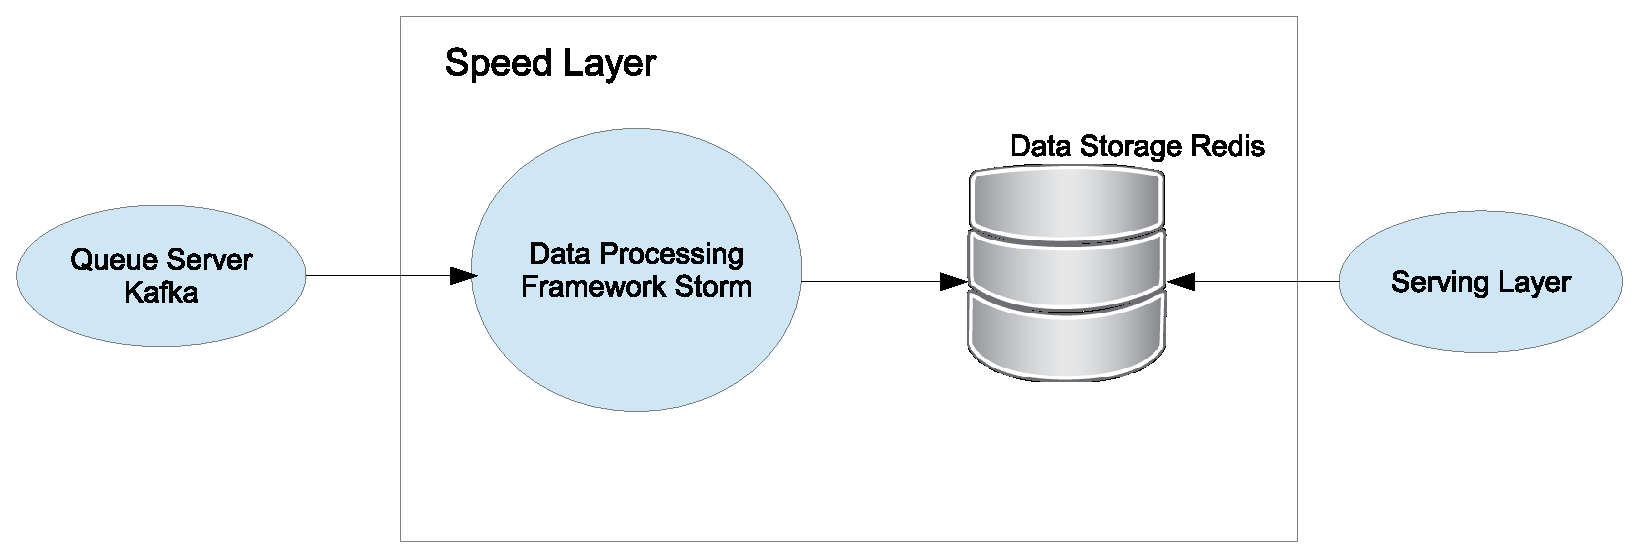
\includegraphics [width=1.0\textwidth]{images/SpeedLayerArchitecture}
  \caption{General structure of our system.}
  \label{fig:SpeedLayerArchitecture}
\end{figure}

\subsection{Data source}

The source of data, that is being processed, is the Kafka queue server \ref{subs:kafka}.
In its turn, it receives data from the outer sources, specifically from smartphones.
There are so far tens of thousends of smartphones, that use Menthal application and send data to the server.
Their number can grow arbitrarily, what requires in essence to have such a complex distributed server.
Smartphones send data to the server in small batches, that contain about fifty events, that happened since the last sending.
Kafka queue server stores this data temporarily, and tries to send it to all consumers, until they acknowledge delivery.
Our system is one of the consumers, and when it receives data, it starts processing. 

For each event type Kafka queue server maintains a dedicated topic.
It is possible then to subscribe for receiving of those events, that are needed for processing.
Events are sent as Avro objects \ref{subs:avro}, and contain meaningful information about what user does on the phone.
In our case we consider event types presented in the Table~\ref{table:event_types}.

\begin{table}[h]
\begin{tabular}{ | l | p{10cm} |}
    \hline
    AppInstall & Contains user id, app name and timestamp. Generated when the user installed a new application. \\ \hline
    AppSession & Contains user id, app name, timestamp and duration. Generated when the user has finished a session of using application. \\ \hline
    CallMissed & Contains user id, timestamp and contact hash. Generated when the user missed a call. Contact hash specifies a contact, that called. \\ \hline
    CallOutgoing & Contains user id, timestamp, contact hash and duration. Generated when the user finished an outgoing call. Contact hash specifies a contact, to that the call was addressed. \\ \hline
    CallReceived & Contains user id, timestamp, contact hash and duration. Generated when the user finished an incoming call. Contact hash specifies a contact, that called. \\ \hline
    DreamingStarted & Contains user id and timestamp. Generated when the phone gone to the dreaming mode. \\ \hline
    DreamingStopped & Contains user id and timestamp. Generated when the phone woke up from the dreaming mode. \\ \hline
    PhoneShutdown & Contains user id and timestamp. Generated when the phone goes off. \\ \hline
    ScreenOff & Contains user id and timestamp. Generated when the phone's screen goes off. \\ \hline
    ScreenOn & Contains user id and timestamp. Generated when the phone's screen goes on. \\ \hline
    ScreenUnlock & Contains user id and timestamp. Generated when the phone's screen is unlocked. \\ \hline
    SmsReceived & Contains user id,  timestamp, contact hash and message length. Generated when an sms is received. Contact hash specifies the contact, from that sms has come. \\ \hline
    SmsSent & Contains user id,  timestamp, contact hash and message length. Generated when an sms is sent. Contact hash specifies the contact, to that sms was sent. \\ \hline
    WindowStateChanged & Contains user id, timestamp, app name and window title. Generated when the new window becomes active. \\
    \hline
\end{tabular}
\caption{Event types and their descriptions}
\label{table:event_types}
\end{table}

\mnote{Kafka spout}
To obtain events from the Kafka queue server, we use \textit{Kafka spouts}.
Kafka spout is the class in the Storm's external class library, that allows to use Kafka queue server as a source of data for processing in the topology.
It listens for messages coming from Kafka in a particular topic.
Each such spout works in a distributed fashion, so that no matter how many events of a particular type will come, we can overcome this simply adding more machines to the cluster.

\subsection{Data processing}

The data processing framework Storm \ref{subs:storm} is the main component of the system.
It receives messages from Kafka queue server, and performs different computations on that data.
Its purpose is to provide different aggregatons on data coming from smartphones.
These aggregations are then stored in the storage system, and can be accessed by the Speed layer for answering queries.

The core of Storm framework is topology.
Topology describes the flow of computational logic.
It contains spouts and bolts, that represent data sources and data processing nodes, respectively.
We have already discussed Kafka spout, that we use for receiving data from the Kafka queue server.

Our topology has simple structure, but nevertheless has many nodes inside.
First of all, for each event type there is dedicated Kafka spout, that receives data from the Kafka queue server.
For that sake each Kafka spout is subscribed for a specific Kafka topic, corresponding to that event type.
When new message comes from the Kafka queue server, Storm runs particular spout on any available cluster node.

There is a dedicated bolt for each event type in our topology.
For each bolt we create a dedicated class, that performs particular processing, depending on what event type is it.
We use Storm's class \lstinline{BaseRichBolt} as a base class for all our bolts.
Our abstract class \lstinline{EventProcessingBolt}, that extends \lstinline{BaseRichBolt}, provides base functionality for all other bolts.
Every particular bolt class implements abstract method \lstinline{processEvent}, given in the class \lstinline{EventProcessingBolt}.
Such class hierarchy allows to add new event types for processing easily.
We just need to create new class, that inherits from \lstinline{EventProcessingBolt} and implements method \lstinline{processEvent}.

Class \lstinline{EventProcessingBolt} has a method \lstinline{getEventProcessingBoltByEventName}, that creates new bolt class by its name.
To achieve such functionality, class \lstinline{EventProcessingBolt} has protected field \lstinline{schemaName}.
It must be initialized in each derived class with the name of this particular event type.
This is useful again for the sake of extensibility, because it let's to leave code of topology initialization the same, no matter how many new event types we add for processing.
The main method of the \lstinline{EventProcessingBolt}, namely \lstinline{execute}, is presented on the Listing~\ref{listing:EventProcessingBolt_execute}.

\begin{lstlisting}[float=h, caption=The main method of the EventProcessingBolt., label=listing:EventProcessingBolt_execute, language=Java]
public void execute(Tuple tuple) {
  try {
    Schema schema = new Schema.Parser().parse(new File(schemaName + ".avsc"));
    DatumReader<GenericRecord> datumReader = new GenericDatumReader<GenericRecord>(schema);
    InputStream in = new ByteArrayInputStream((byte[])tuple.getValue(0));
    GenericRecord record = datumReader.read(null, DecoderFactory.get().jsonDecoder(schema, in));
    processEvent(record);
    _collector.emit(new Values(record));
  } catch (Exception e) {
    System.out.println("Exception raised!");
    System.out.println(e.getMessage());
  }
}
\end{lstlisting}

In the Line 3 we parse the schema of that particular event type.
Then in Lines 4-6 we parse input event to a \lstinline{GenericRecord} object using that schema.
\lstinline{GenericRecord} is an Avro class for representation of Avro objects in memory.
In the Line 7 we call abstract method \lstinline{processEvent}, that executes particular processing depending on what exact bolt class is it.

\lstinline{EventProcessingBolt} holds a reference to an interface \lstinline{EventAggregator}.
This interface provides method for processing all of event types that we consider.
Listing~\ref{listing:EventAggregator} shows the snippet from the definition of that interface.
We implemented exact class \lstinline{RedisEventAggregator} that realizes this interface.
As it states in its name, it works with Redis data storage.

\begin{lstlisting}[float=h, caption=The partial listing of the interface EventAggregator., label=listing:EventAggregator, language=Java]
public interface EventAggregator {
  void processAppSession(long userId, long time, long duration, String appName);
  void processCallMissed(long userId, long time, String contactHash, long timestamp);
  void processScreenOn(long userId, long time);
  void processSmsSent(long userId, long time, String contactHash, int msgLength);
  void processWindowStateChanged(long userId, long time, String appName, String windowTitle);
  ...
}
\end{lstlisting}

To make an example, let us consider one particular bolt class - \lstinline{AppSessionBolt}.
Listing~\ref{listing:AppSessionBolt} presents it.
In the constructor we initialize \lstinline{schemaName} with the name of this event type.
It is useful for creation of bolts by name.
In the method \lstinline{processEvent} we print out given record, then retrieve data fields from it, and pass them to a specific method of the \lstinline{eventAggregator} object, called \lstinline{processAppSession}.

\begin{lstlisting}[float=h, caption=Implementation of AppSessionBolt class., label=listing:AppSessionBolt, language=Java]
public class AppSessionBolt extends EventProcessingBolt {
  public AppSessionBolt() {
    schemaName = "app_session";
  }

  @Override
  protected void processEvent(GenericRecord record) {
    System.out.println(schemaName + "-Bolt: " + record.toString());
    long userId = (long)record.get("userId");
    long time = (long)record.get("time");
    long duration = (long)record.get("duration");
    String appName = record.get("appName").toString();
    eventAggregator.processAppSession(userId,time,duration,appName);
  }
}
\end{lstlisting}

On the events coming from smartphones we do different aggregations.
They will be then taken by the Serving layer for answering queries.
There are three types of aggregation, that we maintain in the data storage: counter, duration, and lenght.
Counter collects the number of events of any particular type.
Duration accumulates the total duration of the continuing action on the smartphone.
Length contains the total length of sms or whatsapp messages, etc.
There is a different logic of how to compute them for these three types of aggregations. 

anomaly detection

\subsection{Data storage}

Data storage Redis \ref{subs:redis} is a place, where all results of computations are kept.
These results are different aggregations, specifically counters, that are stored in the complex data model.
Redis provides simple access to save and then get that data.
Counters, saved in the Redis data storage can be then used by the Speed layer to merge them with the results of batch computations.

redis
keys
access to redis
transactions and pipelining